\setchapterpreamble[u]{\margintoc}
\chapter{Conclusiones}
\labch{conclusions_spanish}
\label{sec:conclusions_spanish}

En este trabajo se han propuesto múltiples metodologías para fusionar la información adquirida por diferentes sensores integrados en un dron. El método de registro de imágenes conocido como "Enhanced Correlation Coefficient" (\acrshort{ecc}), propuesto por Evangelidis y Psarakis \cite{evangelidis_parametric_2008}, se ha utilizado como base para alcanzar un sistema compuesto por múltiples capas de información. Dicho algoritmo no se había explorado aún en teledetección para registrar imágenes con observaciones radiométricas muy diferentes. En esta tesis, se ha mostrado la eficacia de dicho método para fusionar información en el espectro visible e infrarrojo. A partir de aquí, este sistema multicapa se ha extendido a nubes de puntos 3D mucho más fáciles de interpretar y visualizar por operadores humanos. La reconstrucciones de nubes 3D suele llevarse a cabo mediante fotogrametría; no obstante, ésta es bastante proclive a introducir errores geométricos con imágenes de resolución reducida, como las imágenes térmicas y multiespectrales. Además, una resolución tan reducida también deriva en una baja densidad de puntos. Una vez descritos estos inconvenientes, se propone estimar con fotogrametría una nube de puntos de referencia utilizando únicamente imágenes de alta resolución, mientras que el resto de la información se proyecta en dicha nube de puntos. Por tanto, el sistema compuesto por múltiples capas se extiende al 3D. Por otro lado, los hipercubos también se han proyectado sobre nubes de puntos 3D, aunque son muy pocos los trabajos que se enfocan en esta tarea en la literatura. En este caso, el proceso de adquisición de datos es significativamente más peculiar, dado que el sensor funciona escaneando líneas espaciales a lo largo de una distancia considerable. Por tanto, son muy pocas las imágenes obtenidas, y éstas presentan grandes dimensiones. Por tanto, dadas estas peculiaridades, entre las que se incluye un ángulo de visión \textit{nadir}, la extensión al 3D no es tal sino simplemente un mapa de altura en 2.5D. Finalmente, los resultados obtenidos se han empleado en diversas aplicaciones. Las imágenes y nubes de puntos térmicas se han utilizado en la identificación de restos arqueológicos, y por último, las imágenes hiperespectrales se procesaron para dar lugar a un algoritmo de clasificación de diferentes variedades de vid mediante Deep Learning.

Por otro lado, los datos obtenidos mediante sensores reales presentan algunas desventajas, tales como la lentitud del proceso de adquisición así como en las tareas de procesamiento (eliminación de ruido, etiquetado, etc.). Para evitar algunas de estas desventajas, se implementó un simulador \acrshort{lidar} con el fin de obtener conjuntos de datos sintéticos que podrían incluir cualquier tipo de información en cada punto generado. A día de hoy, se ha explorado la generación de imágenes sintéticas mediante Redes Generativas Adversarias (\acrshort{gan}), aunque debido al ámbito limitado de esta tesis, se ha explicado únicamente la simulación de un sensor \acrshort{lidar}.  Dicho simulador se ha empleado para construir grandes conjuntos de datos tanto de misiones aéreas como terrestres. Sobre cada punto se añadió información radiométrica utilizando dos enfoques diferentes. Ambos fueron capaces de producir nubes de puntos con valores de intensidad, mostrando diferencias muy notables entre superficies modeladas con materiales distintos. Posteriormente, la simulación \acrshort{lidar} se aplicó a la optimización de escaneos utilizando metaheurísticas que ayudaron tanto a reducir el número de posiciones como a calcular las posiciones óptimas dentro de un espacio tridimensional.

A nivel técnico, estos tres últimos años me han ayudado a mejorar como investigador. El trabajo realizado ha dado lugar a importantes resultados que han sido publicados en revistas y congresos de primer nivel en el campo de la teledetección, mientras que otros están aún en proceso de revisión. Además, he tenido el placer de participar en trabajos de otros compañeros, que, a pesar de no formar parte de la temática de esta tesis, han contribuido enormemente a aprender mucho más acerca de la informática gráfica.

\section{Resumen de las contribuciones presentadas}

En la primera parte de esta tesis se describió una metodología para corregir y fusionar imágenes procedentes de múltiples sensores. El algoritmo de registro de imágenes conocido como "Enhanced Correlation Coefficient" se utilizó para poder alinear los resultados obtenidos por sensores sensibles a diferentes intervalos de longitud de onda. Se obtuvieron buenos resultados a pesar de las diferencias radiométricas tan significativas que existían entre imágenes, y se utilizó de manera masiva para co-registrar imágenes visibles, multiespectrales e infrarrojas. Además, la eficacia de dicho algoritmo se comprobó utilizando dimensiones de imagen mucho menores, inclusive con mayor desenfoque, y evaluando la correlación final. De hecho, el desenfoque gaussiano permitió reducir significativamente el tiempo de respuesta sin empeorar los resultados obtenidos.

El procedimiento de registro de imágenes se convierte así en el núcleo de esta tesis y se utilizará en los capítulos posteriores relacionados con la fusión de imágenes. A partir de aquí, se extiende dicha fusión al 3D (nubes de puntos). Estas últimas son mejores para aplicaciones específicas que requieren tareas de visualización y de posicionamiento de ciertos detalles que pudieran observarse en el área. Sin embargo, no son tan útiles si la densidad de punto es baja o presentan una geometría incorrecta. Por ello, se describió un procedimiento para la generación de nubes de puntos visibles, térmicas y multiespectrales de grandes dimensiones y con una elevada densidad de puntos. Primero, se generó una nube de puntos \acrshort{rgb} muy densa y de gran tamaño utilizando fotogrametría, mientras que el resto de conjuntos de datos se proyectaron sobre esta nube de puntos densa y de mayor precisión. De este modo se abordaron algunos de los principales inconvenientes de la fotogrametría cuando se aplica sobre imágenes térmicas y multiespectrales. Además, se comparó nuestra solución con software comercial, evidenciando una mejora  en términos de 1) tiempo de respuesta, 2) densidad y 3) tamaño. Por otra parte, la proyección también debe tener en cuenta la oclusión de las superficies para generar información radiométrica fiable. Para lograr esto mismo, se detectó la oclusión utilizando un búfer de profundidad, mientras que las muestras proyectadas se combinaron mediante funciones de agregación y penalización. Estas últimas ayudaron a obtener un color agregado con el objetivo de minimizar la distancia de dicho valor a las muestras iniciales. 

Además de tener en cuenta la oclusión, esta metodología se implementó en la \acrshort{gpu}, tal y como lo haría software comercial como Agisoft Metashape o Pix4Dmapper. Sin embargo, la metodología propuesta obtuvo un tiempo de respuesta mucho menor. Se comprobaron otras mejoras, como la reordenación de la nube de puntos de manera global o local (en pequeños grupos). Los experimentos llevados a cabo mostraron que la reordenación global de una nube de puntos mejoraba significativamente el tiempo de respuesta, incluso considerando el tiempo derivado de la ordenación. Por otro lado, la ordenación local no obtuvo mejores resultados, debido a la sobrecarga derivada de la ordenación + reordenación aleatoria, de tal manera que empeora el tiempo de respuesta siempre y cuando el proceso sólo se ejecute una vez.

La segunda parte de esta tesis también incluye la generación de nubes de puntos hiperespectrales, que, hasta donde sabemos, no se había logrado anteriormente, al menos fuera de laboratorio. Para ello, las imágenes hiperespectrales se fusionaron utilizando como referencia un ortomosaico RGB. Posteriormente, se proyectó la información hiperespectral sobre la voxelización de una nube de puntos 3D, a lo cual hemos hecho referencia como campo de alturas. Por tanto, los resultados se representaban en 2.5D, en lugar de 3D, debido a que los conjuntos de datos hiperespectrales se obtuvieron con un ángulo de visión \textit{nadir}. El tamaño del vóxel se adaptó a la resolución espacial de la imagen, y las imágenes hiperespectrales se solaparon sobre el campo de alturas mediante funciones de agregación y penalización. Debido a la elevada dimensionalidad del hipercubo resultante, éste comprimió en la dimensión radiométrica siguiendo un enfoque basado en \textit{stacks} \cite{graciano_quadstack_2021}. La mayoría de los pasos se implementaron en la \acrshort{gpu}, e incluso así, unos de los principales inconvenientes del hipercubo comprimido era recorrerlo en tiempo real debido a que esto debe resolver de manera iterative para cada píxel. Este inconveniente se resolvió formando las imágenes en múltiples fotogramas. y al igual que en capítulos anteriores, la visualización de nubes de puntos se mejoró utilizando los \textit{compute shaders} de \acrshort{opengl}.

A pesar de componer un sistema multicapa, éste carecía de otras fuentes de información procedentes de sensores de los que no disponíamos, como el sensor \acrshort{lidar}. Por tanto, se propuso un simulador \acrshort{lidar} que permitía resolver las intersecciones con un tiempo de respuesta muy reducido, además de considerar errores sistemáticos y aleatorios descritos en trabajos previos. Dichos errores se derivaban de partículas atmosféricas, superficies con una reflectancia alta, de la altura de vuelo o la pendiente de la superficie medida. La simulación se parametrizó para poder incorporar las especificaciones de cualquier sensor \acrshort{lidar} disponible en el mercado. No obstante, algunos trabajos anteriores ya habían resuelto parcialmente esta simulación con el fin de generar conjuntos de datos \acrshort{lidar} para Deep Learning. Sin embargo, otro factor clave es la utilización de escenarios sintéticos; en este trabajo, estos se generararon de manera procedural para poder obtener un gran número de escenarios diferentes, y por tanto, de nubes de puntos. Los escenarios se etiquetaban relacionando modelos y materiales con etiquetas, todo ello en función del nombre de la superficie, facilitando pues dicha tarea manual. Debido a esto último, los escenarios procedurales son especialmente interesantes dado que sólo deben etiquetarse una única vez, a pesar de dar lugar a muchos escenarios distintos. En cualquier caso, también era posible utilizar escenarios sintéticos constantes, sin modelado procedural. Por último, se comparó el cálculo de intensidad \acrshort{lidar} mediante \acrshort{brdf}s analíticas, como se emplean para el sombreado eficiente en Informática Gráfica, y con \acrshort{brdf}s obtenidas de mediciones reales empleando un goniofotómetro. La comparativa con nubes reales era difícil de establecer, por lo que los experimentos se llevaron a cabo mostrando los histogramas de intensidad de escenarios modelados con diferentes materiales. La simulación \acrshort{lidar} se llevaba a cabo en la \acrshort{gpu} para resolver rápidamente misiones aéreas y terrestres; desde la generación de pulsos \acrshort{lidar} hasta el propio escaneo.

A diferencia de los simuladores \acrshort{lidar} previamente descritos en la literatura, nuestra solución permite llevar a cabo misiones tanto terrestres como aéreas. El primero tipo de simulación es el más habitual, mientras que el segundo apenas se ha descrito con anterioridad. Ambos requieren una trayectoria, definida por el usuario o calculada automáticamente, mientras que las misiones aéreas también emplean diferentes patrones de barrido, entre los que se incluyen el escaneo paralelo, en zigzag y con forma de elipsoide. Además, también se simulan múltiples retornos que son de gran utilidad para eliminar la copa de los árboles y la vegetación de la nube de puntos obtenida. Por último, también se simula el \acrshort{lidar} batimétrico para alcanzar superficies debajo del agua. 

Finalmente, los conjuntos de datos y resultados obtenidos en capítulos anteriores se emplearon en casos de estudio prácticos. En primer lugar, se procesaron y corrigieron las imágenes hiperespectrales para su posterior clasificación en variedades de viñedo tanto rojo como blanco. Las técnicas tradicionales, basadas en la correlación del perfil espectral, no se ajustaban a la clasificación de perfiles muy similares, y por tanto, se utilizaron redes neuronales para tal tarea. Se resolvió esta aplicación utilizando capas exploradas en el estado del arte actual, como Inception o capas de atención espacial. Los hipercubos se dividían en pequeños bloques, cuyo tamaño se evaluó durante la experimentación, y se reducían a una sola etiqueta; por lo tanto, la clasificación de cada muestra dependía de un conjunto de píxeles a su alrededor. No sólo se comprobó la red propuesta sobre datos de dron, sino también sobre datos de satélite, obteniendo igualmente una precisión muy alta. Por último, se aplicaron imágenes y nubes de puntos térmicas a la inspección de un yacimiento arqueológico, donde se detectaron dos zonas anómalas que podrían corresponder a la ubicación de dos torres aún no exploradas. 

\section{Trabajo futuro}

La teledetección y la inteligencia artificial se encuentran en constante evolución, y a pesar de ello, existen algunos trabajos futuros que debieran explorarse a partir de esta tesis:
\begin{itemize}
    \item El registro de imágenes se llevó a cabo utilizando hardware que no estaba orientado a altas prestaciones, y por lo tanto, se exploraron alternativas para mejor la eficiencia como la reducción de tamaño de imágenes o su desenfoque. No obstante, una alternativa consiste en explorar un esquema piramidal que, partiendo de un tamaño muy reducido, permita obtener una transformación inicial con menor nivel de detalle (pero capaz de identificar grandes cambios). A medida que se incrementa el tamaño de imagen, el nivel de detalle del registro es mayor, pero los cambios son de menor entidad, y por tanto, se estiman en un menor tiempo de respuesta.  Además de reducir la latencia, este enfoque también podría ayudar a emparejar imágenes con diferencias mucho mayores.
    \item El registro de imágenes formaba parte de la fase de lectura y procesamiento de datos en las comparaciones establecidas con software de fotogrametría. Por lo tanto, esta etapa podría acelerarse aún más implementando \acrshort{ecc} en la \acrshort{gpu}.
    \item La generación de nubes de puntos 3D con una densidad de puntos muy elevada, con información \acrshort{rgb}, térmica y multiespectral; sin embargo, las nubes de puntos con una dimensionalidad tan elevada son también más difíciles de renderizar en tiempo real. Aunque el renderizado utilizando compute-shader ayudó considerablemente a reducir a la latencia \cite{schutz_rendering_2021}, podría mejorarse aún más con diferentes niveles de detalle (\acrshort{lod}) \cite{schutz_gpu-accelerated_2023}. Del mismo modo, podría ayudar a renderizar hipercubos comprimidos, dado que uno de los principales inconvenientes encontrados fue un renderizado mucho menos eficiente que de costumbre.
    \item La compresión de hipercubos se implementó reduciendo la resolución radiométrica mediante una representación basada en pilas, mientras que la compresión espacial no obtuvo buenos resultados debido a la gran variabilidad de los datos en la dimensión espacial. En lugar de una representación basada en pilas, la compresión podría llevarse a cabo en la dimensión espacial, de mucho mayor tamaño que la dimensión espectral. 
    \item La optimización \acrshort{lidar} se exploró en la identificación de ubicaciones óptimas para el escaneo con \acrshort{lidar} terrestre. Sin embargo, hay otros tipos de \acrshort{lidar} que podría también explorarse, especialmente aquellos que requiren una trayectoria. De esta manera, las optimizaciones basadas en poblaciones podrían ser de gran utilidad para este tipo de trayectorias \cite{roberge_fast_2018}. La optimización de \acrshort{lidar} aéreo también podría explorarse para determinar cuál es la configuración óptima para escanear  una escena con una densidad elevada a partir de un \acrshort{dsm}, incluyendo la trayectoria.
    \item Una propuesta similar consiste en evaluar misiones de dron calculando una trayectoria que garantice ciertos requisitos de solapamiento y cobertura en función del tiempo, la altitud y la velocidad de vuelo, entre otros factores. Este mismo problema se ha estudiado para misiones de dron genéricas \cite{pessacg_simplifying_2022}; no obstante, podría mejorarse aún más en función de la geometría de la escena, representada mediante modelos rápidamente esbozados. Esto podría ser de especial interés para vuelos que requieren observaciones oblicuas, con un ángulo configurable por el usuario. 
    \item Hasta ahora, las simulaciones \acrshort{lidar} se han utilizado para generar grandes conjuntos de datos ya etiquetados. Sin embargo, los conjuntos de datos generados deben comprobarse en tareas de clasificación y segmentación mediante Deep Learning, con el fin de verificar que los conjuntos de datos de entrada podría sustituirse, al menos de manera parcial, por datos sintéticos. Nótese que algunos de los errores simulados se omiten mediante la voxelización de las nubes de puntos \cite{hackel_semantic3d_2017, behley_towards_2021}. Por tanto, es necesario discernir si estos conjuntos de datos sintéticos son lo suficientemente similares a los conjuntos de datos reales. 
    \item Además de \acrshort{lidar}, hay otros sensores basados en imágenes que pueden ser simulados mediante redes generativas adversaria (Generative Adversarial Networks). Éstas permiten generar conjuntos de datos no supervisados que van desde obras de arte hasta datos en forma de texto. Por ejemplo, podrían construirse imágenes térmicas a partir de imágenes visibles con el fin de crear conjuntos de datos más amplios. El estado del arte en este campo aún no ha logrado con éxito esta tarea, empleando únicamente información visible como entrada \cite{li_multi-branch_2019, li_i-gans_2021, kniaz_thermalgan_2019, ozkanoglu_infragan_2022, yi_cycle_2023}. Sin embargo, esta tarea podría ayudarse de anotaciones semánticas que permitan identificar superficies distintas, las cuales a su vez pueden producir información radiométrica diferente.
    \item La clasificación de variedades de vid se resolvió con Deep Learning; sin embargo, este modelo podría mejorarse integrando más variedades y recopilando más conjuntos de datos en diferentes etapas del año. Además, existen otros enfoques interesantes para abordar esta misma tarea, desde la clasificación multi-instancia \cite{meerdink_multitarget_2022} hasta el aprendizaje por comparación \cite{guan_spatial-spectral_2022}. 
\end{itemize}

% Añadir referencia
\begin{figure}
    \centering
    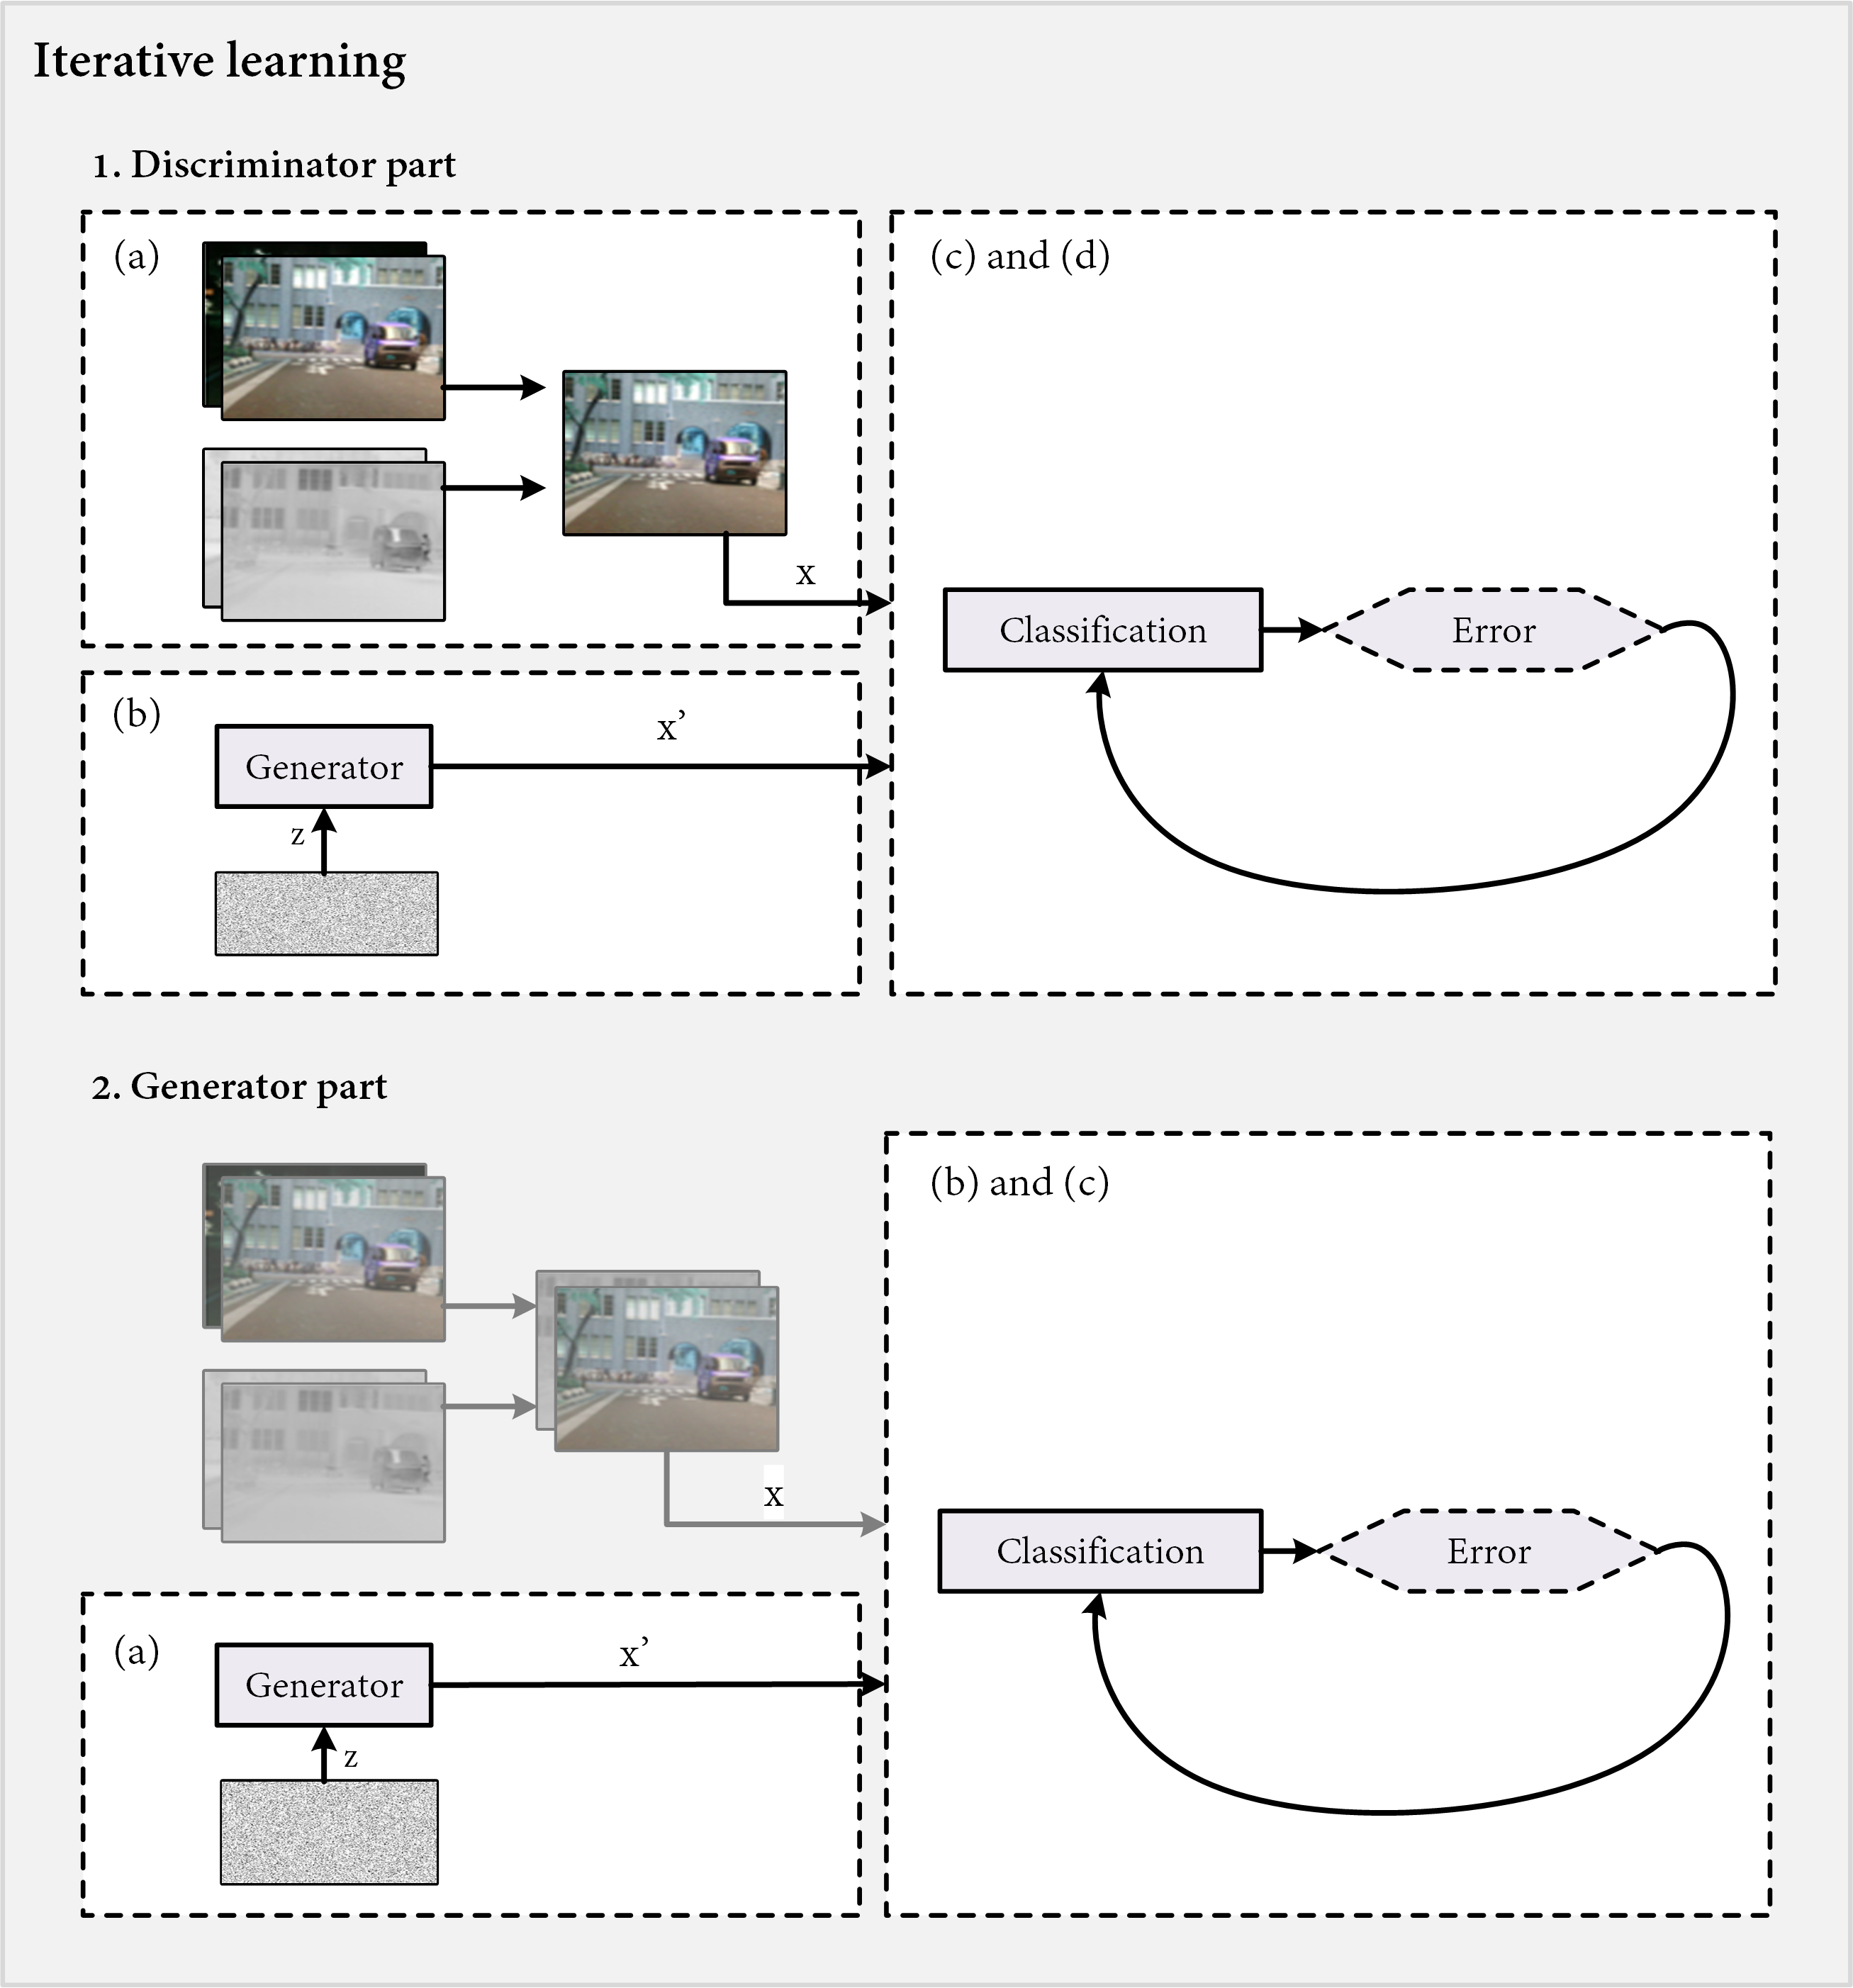
\includegraphics[width=\linewidth]{figs/conclusions/gan.png}
    \caption{Esquema de una red generativa adversaria, compuesto a su vez por dos modelos diferentes: generador y discriminador. El primero debe entrenar para producir datos tan realistas como sea posible, mientras el segundo debe discernir, con la mayor eficacia posible, si los datos de entrada son reales o no.}
    \label{fig:conclusiones_gan}
\end{figure}